\documentclass{article}%
\usepackage[T1]{fontenc}%
\usepackage[utf8]{inputenc}%
\usepackage{lmodern}%
\usepackage{textcomp}%
\usepackage{lastpage}%
\usepackage[head=40pt,margin=0.5in,bottom=0.6in]{geometry}%
\usepackage{graphicx}%
%
\title{\textbf{Trabajadores exigieron a la Defensoría la liberación de Rubén González}}%
\author{CARLOS SEIJAS MENESES}%
\date{04/12/2018}%
%
\begin{document}%
\normalsize%
\maketitle%
\textbf{URL: }%
http://www.el{-}nacional.com/noticias/politica/trabajadores{-}exigieron{-}defensoria{-}liberacion{-}ruben{-}gonzalez\_262039\newline%
%
\textbf{Periodico: }%
EN, %
ID: %
262039, %
Seccion: %
Política\newline%
%
\textbf{Palabras Claves: }%
NO\_TIENE\newline%
%
\textbf{Derecho: }%
1.2%
, Otros Derechos: %
1.10%
, Sub Derechos: %
1.2.2, 1.10.2.1%
\newline%
%
\textbf{EP: }%
SI\newline%
\newline%
%
\textbf{\textit{Sindicalistas consignaron un documento en el que piden que se “vele por los derechos humanos” del dirigente, procesado en un tribunal militar}}%
\newline%
\newline%
%
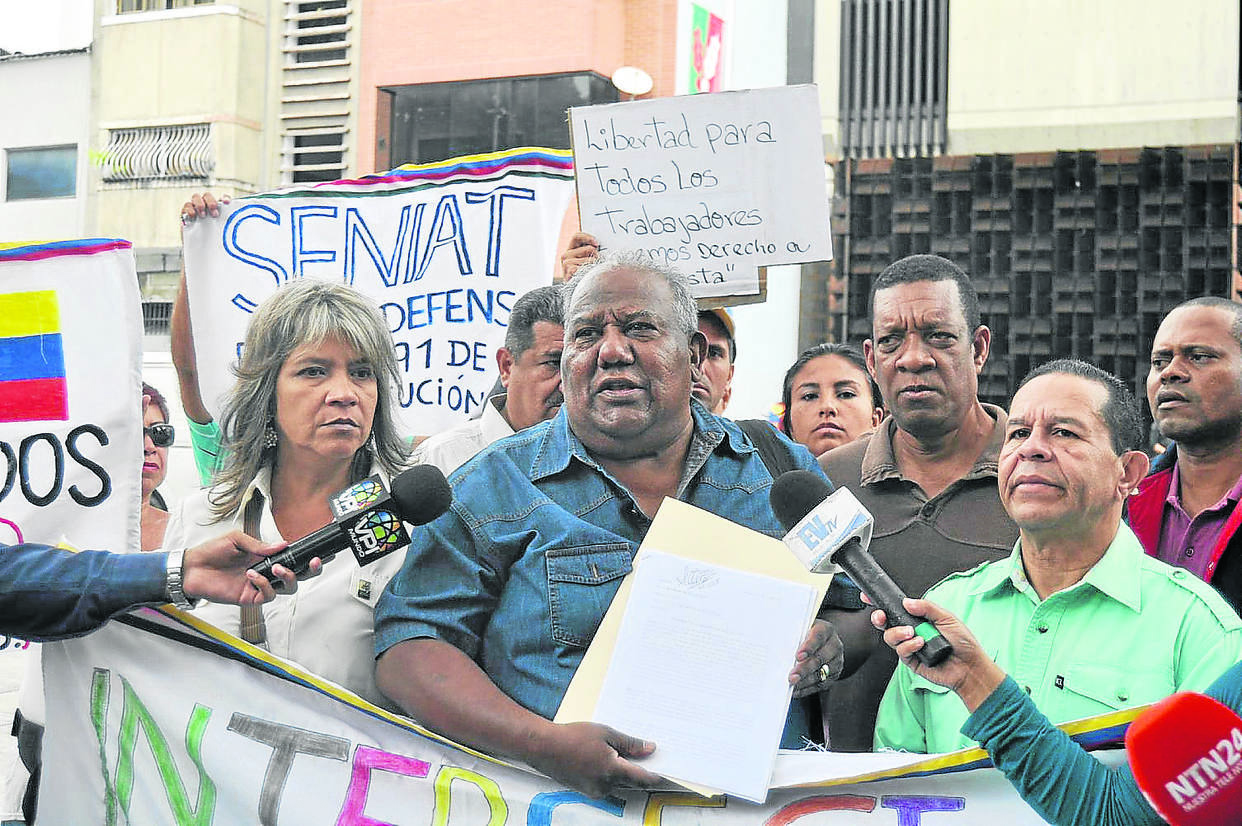
\includegraphics[width=300px]{92.jpg}%
\newline%
%
A cuatro días de que un tribunal militar en el estado Monagas sentenció prisión para Rubén González, secretario general del Sindicato de Ferrominera, y luego~trasladado a la cárcel de~La Pica, dirigentes sindicales en Caracas fueron a~la Defensoría~del Pueblo, avenida Urdaneta, para consignar un documento en el que le piden al funcionario Alfredo Ruiz Angulo que “vele por los derechos humanos” del dirigente, violados al ser procesado en jurisdicciones militares. También exigieron su liberación inmediata. Le fueron imputados ataque al centinela, ultraje al centinela y ultraje a~la Fuerza Armada~Nacional Bolivariana.%
\newline%
%
“¡El compañero Rubén González no cometió ningún delito! El defensor del pueblo está obligado, como lo establece el artículo 281 de~la Constitución, a ser garante del compañero”, expresó Juan Véliz, presidente del Sindicato de Trabajadores de~la Industria~de Telecomunicaciones, Similares y Conexos del Distrito Capital, uno de los dirigentes~firmantes. “Si el Ejecutivo pensó que esposando a Rubén en el piso nos iba a aminorar, todo lo contrario, está obligando a la clase trabajadora a organizarse de la mejor manera y a que la lucha continúe, incluso en el mes navideño”, añadió.%
\newline%
%
A las 11:13 am dirigentes sindicales, entre ellos Véliz, Pablo Zambrano, de Fetrasalud, y Marlene Sifontes, de Sunep{-}Inparques, le entregaron el documento al abogado Ángel Cartaya, consultor jurídico de~la Defensoría.%
\newline%
%
Sindicalistas han denunciado que González pasó la primera noche en la cárcel de~La Pica~esposado de pies y manos en el piso de un pasillo, y que el sábado a las 9:30 am guardias nacionales le quitaron las esposas enfrente de familiares y trabajadores~que tuvieron acceso a la prisión.%
\newline%
%
Degraín Marichales, delegado de Sintraferrominera, aseguró que el domingo a la 1:00 pm encontró al dirigente sindical en de una celda de reclusión. “Lo vi un poco quebrantado de salud. Rubén está preso por cuestiones políticas. ¿Cuándo a un civil lo han presentado en un tribunal militar con cargos militares?”, preguntó.%
\newline%
%
También denunció que el sábado a las 5:00 pm trasladaron a dos de los nueve trabajadores de Ferrominera, presos en las colonias móviles de El Dorado desde el jueves en la tarde, al Hospital Américo Babó, donde les hicieron pruebas y exámenes físicos debido a que guardias nacionales los golpearon dentro de la cárcel. El martes pasado en la mañana~la Dirección Generalde Contrainteligencia Militar detuvo a Douglas Álvarez, Yonney Monsalve, Alexis Perdomo, Exddy Perdomo, Francisco Perdomo, Pedro Calzadilla, Argenis Dasilva, Tony Briceño y a José Jaime, que protestaban en el portón IV de la empresa estatal.%
\newline%
%
Trabajadores y dirigentes de todas las empresas básicas de Guayana también~se movilizaron el lunes en la mañana. A las 8:00 am~salieron en caravana del elevado de~Alcasa, donde se encuentran las compañías estatales, hacia el centro de la ciudad de Puerto Ordaz “para denunciar el maltrato que sufren González y los demás compañeros detenidos”, afirmó~ Marichales.%
\newline%
%
Algunos trabajadores, que se trasladaban en un vehículo, llevaban pancartas de cartón en las que se leían los mensajes: “La privatización es miseria y hambre para los pueblos” y “Libertad para Rubén González y los trabajadores de Ferrominera”.%
\newline%
%
\end{document}